\section{Einleitung}
\rhead{Einleitung}

Diese Arbeit befasst sich damit, das in Kapitel \ref{chapter:thc} entwickelte 2-Box Modell zur Simulation der Thermohalinen Zirkulation zu einem 3-Box Modell zu erweitern. Mit diesem erweiterten Modell soll dann versucht werden, reale Meeresströmungen zu simulieren. Weiter wird der Einfluss der Klimaerwärmung auf diese Strömungen untersucht und mit anderen, weiter entwickelten Modellen verglichen.

\section{Thermohaline Zirkulation, was ist das?}
\rhead{Thermohaline Zirkulation, was ist das?}

Die hier als THC abgekürzte thermohaline Zirkulation ist eine weltumspannende Meeresströmung.
Diese Strömung sorgt für eine Durchmischung der verschiedenen Ozeane und den damit enthaltenen Energie- und Nährstoffaustausch. 
Die Auswirkung dieses Energieaustausches sind spürbar. So heizt zum Beispiel der Golfstrom, welcher auch zu dieser Strömung gehört, Nordeuropa um mehrere Grad auf.

Doch wie entsteht diese Strömung? 
Diese Problem wurde bereits in Kapitel \ref{chapter:thc} behandelt, darum hier nur eine kurze Zusammenfassung. 



\subsection{Einflussfaktoren}
Es gibt viele Faktoren die zur Entstehung und Veränderung dieser Strömungen beitragen. Dazu gehören die Verteilung der Kontinente, die Corioliskraft, die Wasserdichte und auch Wetter und Winde. Hier gehen wir jedoch nur auf den Einfluss der Wasserdichte ein.
Die Verteilung der Kontinente und auch die Corioliskraft ändern sich nicht und können daher als konstant betrachtet werden. Wind und Wetter werden weggelassen, da ihr Einfluss nur schwer vorherzusagen ist und sie schnell ändern können. Mit dem im Rahmen dieser Arbeit verwendeten Simulationsmodell lassen sich diese Komponenten auch gar nicht darstellen.

\subsection{Dichte}
Die THC wird hauptsächlich durch Dichteunterschiede im Wasser hervorgerufen.
Relativ zur Umgebung sinkt dichtes Wasser ab und weniger dichtes Wasser steigt auf. Die Wasserdichte wird hauptsächlich durch Temperatur und Salzgehalt des Wassers beeinflusst.

Durch einen hohen Salzgehalt wird das Wasser dichter und beginnt zu sinken. Die Temperatur hat einen andersartigen Einfluss, bis $5^\circ\text{C}$ steigt die Dichte des Wassers mit der Temperatur. Ab diesen $5^\circ\text{C}$ ist der Einfluss umgekehrt und die Dichte sinkt wenn die Temperatur steigt. Dieser Effekt hilft auch dabei, dass Eis auf Wasser schwimmt.

Wenn an einem Ort dichtes Wasser absinkt, muss an der Oberfläche anderes Wasser nachfliessen. Dies erzeugt eine Oberflächenströmung. Wenn am Meeresgrund die Dichte des Tiefenwassers reduziert wird, beginnt es aufzusteigen. Dort muss daraufhin Tiefenwasser nachfliessen. Kombiniert entsteht so ein Kreislauf. Skaliert man dies auf Weltmeergrösse, ist die thermohaline Zirkulation beschrieben. Die Einflüsse, welche das Wasser an bestimmten Stellen aufsteigen und absinken lassen, werden später erläutert. 
In Abbildung \ref{thermohalin:graph-salinity} ist der Zusammenhang zwischen Dichte und Salinität dargestellt, in Abbildung \ref{thermohalin:graph-temp} die Abhängigkeit der Dichte von der Temperatur.

\begin{figure}
	\centering
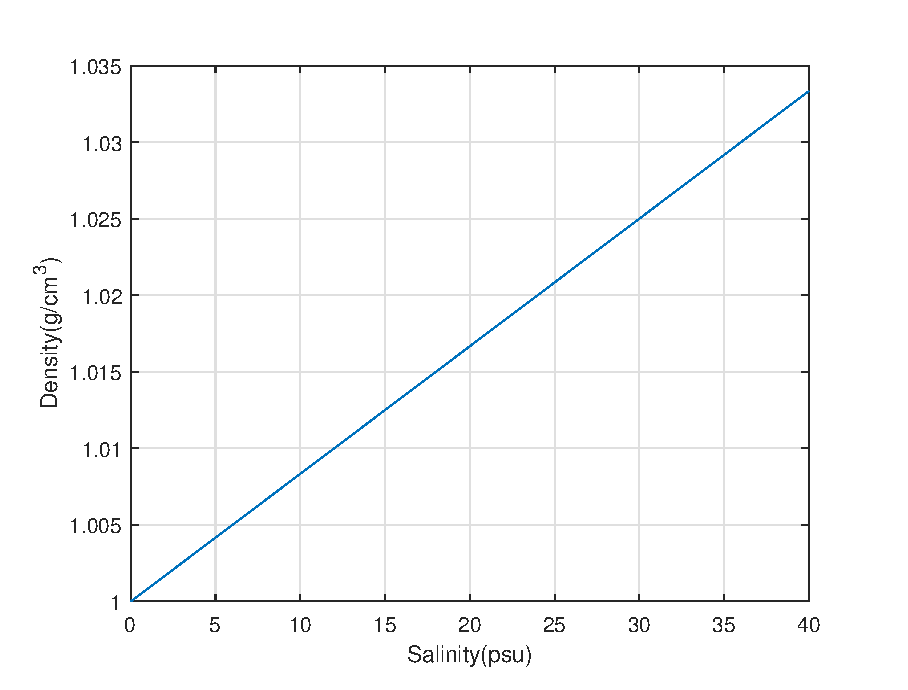
\includegraphics[width=12cm]{thermohalin/Code/graphs/graph_salinity.eps}
\caption{Dichteänderung abhängig vom Salzgehalt\label{thermohalin:graph-salinity}}
\end{figure}
\begin{figure}
	\centering
	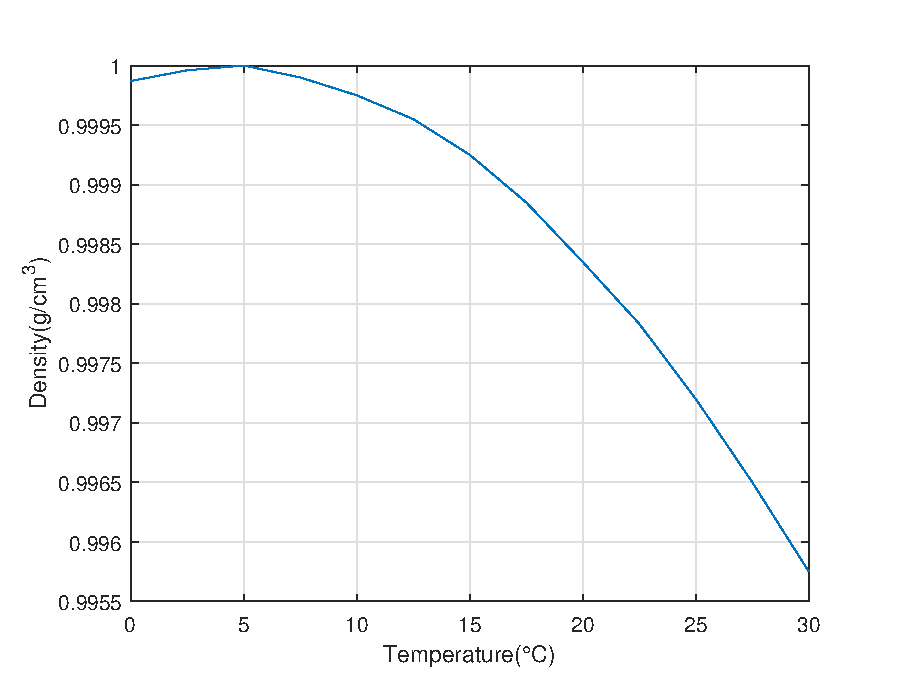
\includegraphics[width=12cm]{thermohalin/Code/graphs/graph_temp.eps}
	\caption{Dichteänderung abhängig von der Temperatur\label{thermohalin:graph-temp}}
\end{figure}

Diese Einflüsse werden in einer Gleichung  
 \begin{equation}
 \varrho
 =
 \varrho_0(1-\alpha(T-T_0)+\beta(S-S_0))
 \label{thermohalin:Dichte}
 \end{equation} 
zusammengefasst, mit welcher sich die Dichte des Wassers berechnen lässt.
Damit lassen sich später über einen Dichteunterschied Wasserströme bestimmen.
Weitere Details zur grundlegenden Funktion der Simulation und die Erklärung der Modellgleichungen sind in Kapitel \ref{skript:thc:modell-gleichungen} zu finden.


\section{Golfstrom}
\rhead{Golfstrom}

Da die Simulation des weltumspannenden THC viel zu umfangreich und kompliziert ist, beschränken wir uns hier auf den Golfstrom.
Der Golfstrom eignet sich bestens zur Simulation, da er sich grob in drei Regionen aufteilen lässt und so gut in das Modell passt. Zusätzlich ist es der Strom, welcher Nordeuropa warm hält. Dies hat auch für die Schweiz eine grosse Bedeutung.

Zusätzlich zur grundlegenden Simulation des Golfstroms wird auch die Reaktion dieser Simulation bei veränderten Umweltparametern betrachtet. Dies, um herauszufinden, ob sich mit dieser Simulation auch Veränderungen durch den Klimawandel darstellen lassen. Abbildung \ref{thermohalin:Deep-Ocean-Currents} enthält eine Darstellung des THC in welcher der Golfstrom hervorgehoben ist. 

\begin{figure}
	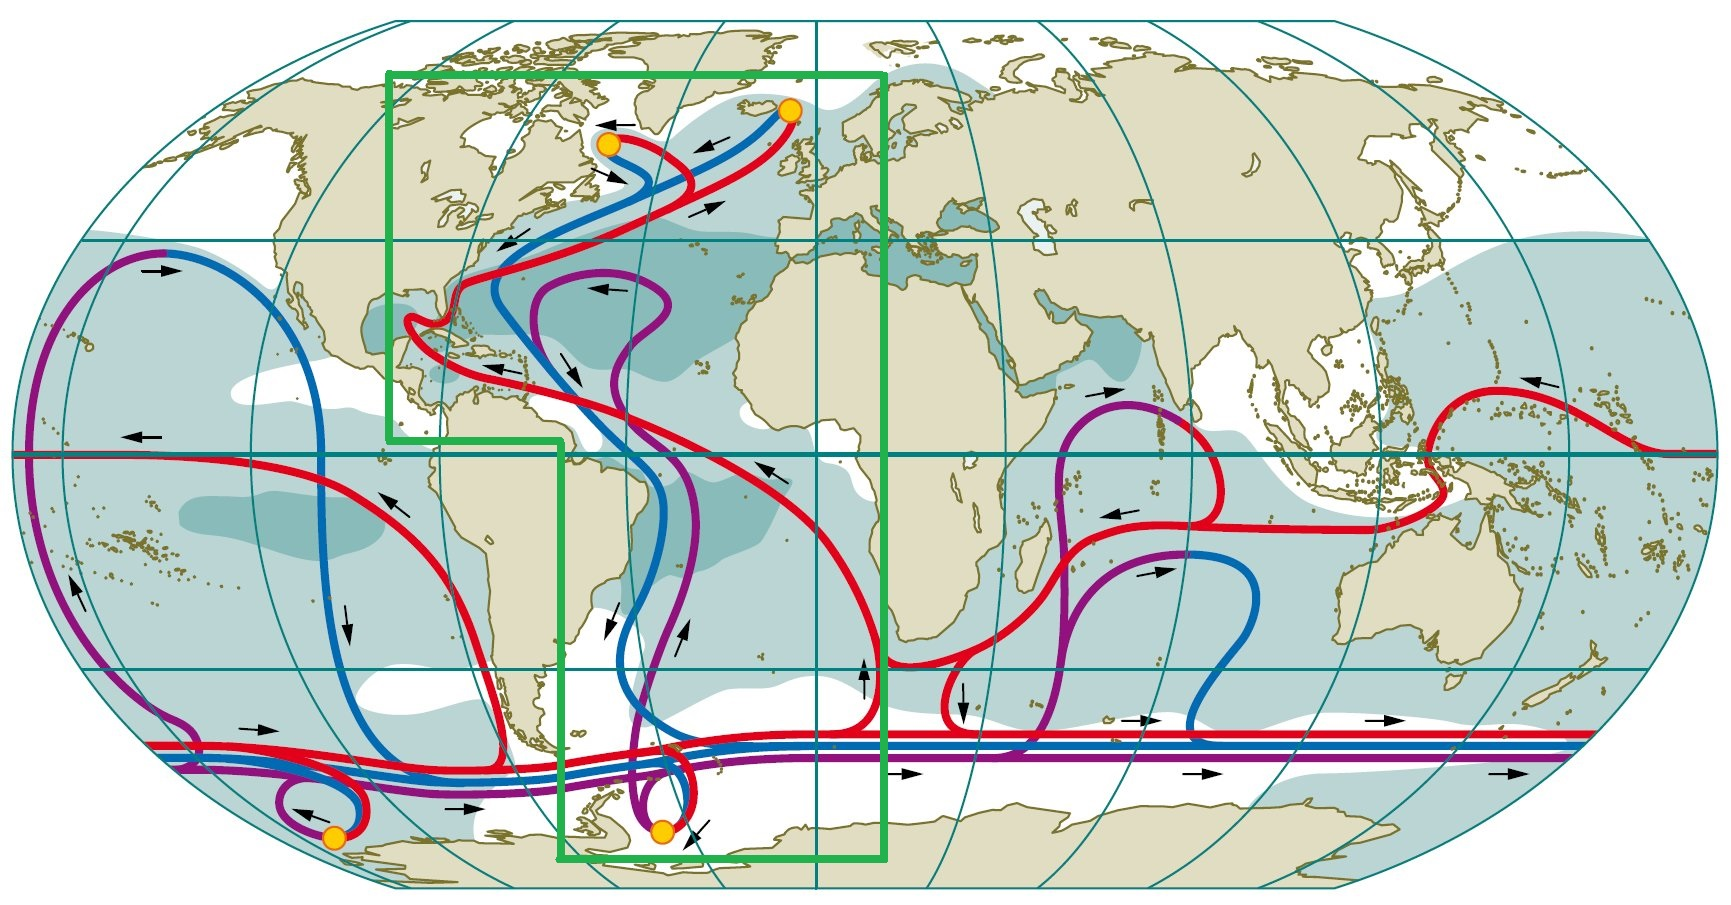
\includegraphics[width=12cm]{thermohalin/Bilder/Deep-Ocean-Currents2.jpg}
	\centering
	\caption{Golfstrom als Teil der Thermohalinen Zirkulation\label{thermohalin:Deep-Ocean-Currents}}
\end{figure}



\subsection{Kreislauf}

Der Golfstrom ist ein Kreislauf und hat keinen Ursprung, deswegen kann mit der Beschreibung an einem beliebigen Ort gestartet werden. Im Golf von Mexiko wird von der Äquatorsonne aufgewärmtes Wasser von Winden und der Erdrotation nach Norden getrieben. Während das warme Wasser an Europa vorbeifliesst gibt es einen Teil seiner gespeicherten Energie ab und wärmt so den Kontinent auf.
Auf dem Weg kühlt das Wasser langsam ab und wird durch die fortlaufende Verdunstung immer salzhaltiger. Da der relative Einfluss der Salinität grösser ist als der, der Temperatur, beginnt das Wasser im Norden, durch die nun hohe Dichte, abzusinken. Das abgesunkene Wasser treibt dem Grund des Meeres entlang bis zum Südpol. Aufgrund der dort anderen Temperatur- und Salzverhältnisse steigt es wieder auf und fliesst in Richtung Atlantik und Mexiko. Somit ist der Kreislauf geschlossen.

\subsection{Einfluss des Klimawandels}\label{thermohalin:EinflussKlimawandel}

Um den Einfluss des Klimawandels auf den Golfstrom zu verstehen, müssen verschiedene Schlüsselstellen betrachtet werden.
Ein Punkt ist das Kap der guten Hoffnungen an der südlichen Spitze Afrikas.
Wie in Abbildung \ref{thermohalin:Deep-Ocean-Currents} ersichtlich ist, befindet sich dort eine Kreuzung.
Der Golfstrom setzt sich dort aus Wasser aus dem indischen Ozean und aus Wasser des Zirkumpolarstromes zusammen. Der conveyor Belt ist eine riesige Strömung welche die Antarktis umschliesst und auch Förderband genannt wird.
Dort stellt sich auch die Frage, in welcher Richtung der Indische Ozean und der Atlantik ihr Salz austauschen und ob überhaupt. Wenn der Golfstrom nicht kontinuierlich mit Salz versorgt wird, ist es dem Wasser am Nordpol nicht mehr möglich zu sinken. Eine leichte Veränderung der Salzbilanz durch eine Störung der Salzzufuhr, könnte den Golfstrom zum Erliegen bringen. Hier gehen die Meinungen von Forschern jedoch auseinander. Salzmessungen im offenen Meer sind sehr schwierig und die Resultate mit Vorsicht zu geniessen.
Im Moment zeigen diese jedoch, dass der Golfstrom weiter Salz in den Atlantik importiert und sich so selber am Leben erhält. Dies könnte sich jedoch durch den Klimawandel ändern. Die Mechanismen der Salzverteilung sind noch nicht komplett verstanden, doch sie lassen sich mit dem aktuellen Klima in Verbindung bringen. Die weltweiten Strömungen sind ein kompliziertes und fragiles System das leicht aus dem Gleichgewicht gebracht werden kann. 

Zusätzlich spielt noch die Erhöhung des CO2-Gehaltes in der Luft und die damit einhergehende Klimaerwärmung eine wichtige Rolle. Sie hat zwei direkte Auswirkungen auf den Golfstrom:

\begin{itemize}
	\item Durch die Erhöhung der Lufttemperatur kann das Wasser auf dem Weg in den Norden nicht mehr genug abkühlen, um danach abzusinken.
	\item Das Abschmelzen der Polkappen, welches viel Frischwasser freisetzt, kann die Salzkonzentration so weit verringern, dass das Wasser aufgrund der reduzierten Dichte nicht mehr absinken kann.
\end{itemize}
Diese beiden Prozesse wären bereits einzeln in der Lage den Golfstrom zu stören, doch zusammen ist die Wirkung noch gravierender.

Laut einer Studie des Forschers Liu Wei von der Universität Yale vom 2. Jan. 2017 \cite{thermohalin:liuwei} könnte dieses Szenario in den nächsten 300 Jahren tatsächlich eintreten. Sie haben den Golfstrom mit der doppelten $\text{CO}_2$ Konzentration wie vor Industrialisierungsbeginn simuliert, also mit einer Konzentration vom $560\text{ppm}$. Die Resultate waren dramatisch. Innert 100 Jahren würde der Strom um einen Drittel abnehmen, und innert 300 Jahren ganz stoppen. Momentan ist die Lage noch nicht so schlimm da die aktuelle $\text{CO}_2$ Konzentration ca. $403\text{ppm}$ \cite{thermohalin:co2} beträgt. Wenn die Konzentration aber weiter so steigt wie zur Zeit, wären wir bereits in 31 Jahren so weit .

\subsection{Folgen}

Was passiert, wenn der Golfstrom zum Erliegen kommt, oder sogar seine Richtung ändert?
Der Katastrophenfilm \texttt{\em{The day after tomorrow}} von Roland Emmerich zeigt auf eindrückliche Weise, was in so einem Fall passieren könnte. 

Die Handlung des Filmes ist folgende: Immer mehr Forscher warnen vor einem drastischen Klimawandel. Sie glauben, dass der Golfstrom wegen der abschmelzenden Polkappen abkühlen und zum Stillstand kommen könnte, was eine neue Eiszeit zur Folge hätte. Zusätzlich hat ein Forscherteam eine Modell entwickelt, welches diese Ereignisse nur wenige Wochen in der Zukunft voraussagt. Zu diesem Zeitpunkt melden bereits erste Bojen rasant absinkende Wassertemperaturen vor der amerikanischen Küste. Innerhalb kürzester Zeit treffen dann Katastrophenmeldungen von überall ein. Neu-Dehli versinkt im Schnee, Tokyo leidet unter Hagelschauern, Los Angeles wird von Tornados zerstört und Superstürme entstehen über Europa, Russland und den USA. 
Innert weniger Tage versinkt die ganze Welt in einer neuen Eiszeit. 

Das ist natürlich übertrieben dargestellt. Doch falls der Golfstrom stoppt, würde Nordeuropa, trotz Klimaerwärmung, um einige Grad kälter werden. Es gibt noch weitere Folgen, doch diese lassen sich nicht so einfach abschätzen, da das Klima ein chaotisches System ist, welches sich nur schwer vorhersagen lässt.

